%%%%%%%%%%%%%%%%%%%%%%%%%%%%%%%%%%%%%%%%%%%%%%%%%%%%%%
% A Beamer template for University of Wollongong     %
% Based on THU beamer theme                          %
% Author: Qiuyu Lu                                   %
% Date: July 2024                                    %
% LPPL Licensed.                                     %
%%%%%%%%%%%%%%%%%%%%%%%%%%%%%%%%%%%%%%%%%%%%%%%%%%%%%%

\documentclass[serif, aspectratio=169]{beamer}
%\documentclass[serif]{beamer}  % for 4:3 ratio
\usepackage[T1]{fontenc} 
\usepackage{fourier} % see "http://faq.ktug.org/wiki/uploads/MathFonts.pdf" for other options
\usepackage{hyperref}
\usepackage{latexsym,amsmath,xcolor,multicol,booktabs,calligra}
\usepackage{graphicx,pstricks,listings,stackengine}
\usepackage{lipsum}
% \usepackage{inputenc}
\usepackage{csquotes}

\usepackage[english]{babel}
\usepackage[newfloat]{minted}
% \setminted{
%   breaklines=true,
%   breakbytoken=true,
%   breakbytokenanywhere=true,
%   fontsize=\small
% }
% \renewcommand{\theFancyVerbLine}{\textcolor{gray}{\arabic{FancyVerbLine}}}

\usepackage[backend=biber,style=ieee,autocite=inline]{biblatex}
% Note: You need a ref.bib file for this to compile
% \addbibresource{ref.bib} % Use this if you have a ref.bib file
\bibliography{ref.bib}
\DefineBibliographyStrings{english}{%
  bibliography = {References},}

\let\oldcite\cite
\renewcommand{\cite}[2][]{\mbox{\oldcite[#1]{#2}}}
  
\author[Danko]{Danila Danko, MS-SE \inst{1} \and \newline \newline {Supervisor: Nikolai Kudasov \inst{1}}}
\title{A Tutorial Implementation of a Lambda Calculus with
Parametric Predicative Arbitrary-Rank Polymorphism}

\institute{
    \inst{1}Innopolis University
}
\date{\small \today}

\usepackage{styling}

% defs
\def\cmd#1{\texttt{\color{red}\footnotesize $\backslash$#1}}
\def\env#1{\texttt{\color{blue}\footnotesize #1}}
\definecolor{deepblue}{rgb}{0,0,0.5}
\definecolor{deepred}{RGB}{153,0,0}
\definecolor{deepgreen}{rgb}{0,0.5,0}
\definecolor{halfgray}{gray}{0.55}

\lstset{
    basicstyle=\ttfamily\small,
    keywordstyle=\bfseries\color{deepblue},
    emphstyle=\ttfamily\color{deepred},    % Custom highlighting style
    stringstyle=\color{deepgreen},
    numbers=left,
    numberstyle=\small\color{halfgray},
    rulesepcolor=\color{red!20!green!20!blue!20},
    frame=shadowbox,
}

\begin{document}

\begin{frame}
  \titlepage
\end{frame}

\begin{frame}{Outline}
  \tableofcontents
\end{frame}

\section{Motivation and Problem}

\begin{frame}[containsverbatim]{The Magic of Modern Type Systems}
  \begin{columns}[T]
    \begin{column}{0.5\textwidth}
      \begin{itemize}
        \item Modern functional languages like Haskell have powerful type systems.
        \item One feature is \textbf{arbitrary-rank polymorphism}, allowing polymorphic functions as arguments.
        \item This enables highly generic and safe code, but its implementation can feel like magic.
        \item \textit{How do compilers like GHC handle this?}
      \end{itemize}
    \end{column}
    \begin{column}{0.5\textwidth}
      \begin{minted}{haskell}
-- Pass a polymorphic function 
-- 'myShow' as an argument
let
  applyMyShow =
    (\x. \y. x y) ::
      forall a.
        (forall b. b -> String) 
           -> a -> String
in
let
  myShow = \x. "Hello"
in
  applyMyShow myShow
            \end{minted}
    \end{column}
  \end{columns}
\end{frame}

\begin{frame}{The Problem: A Pedagogical Gap}
  There is a steep learning curve for understanding how arbitrary-rank polymorphism is implemented.
  \begin{columns}[T]
    \begin{column}{0.45\textwidth}
      \textbf{Foundational Papers}
      \begin{itemize}
        \item Seminal work like \textit{Peyton Jones et al. (2007)} is theoretically dense.
        \item Describes an \textbf{eager unification} algorithm, which is conceptually different from modern practice.
      \end{itemize}
    \end{column}
    \begin{column}{0.55\textwidth}
      \textbf{Production Compilers (GHC)}
      \begin{itemize}
        \item Huge, highly-optimized codebase.
        \item Uses a modern \textbf{constraint-based} architecture, a significant evolution from the papers.
        \item Difficult for a newcomer to trace the connection between theory and implementation.
      \end{itemize}
    \end{column}
  \end{columns}
  \vspace{1em}
  \begin{alertblock}{The Gap}
    We need a "middle ground": a resource more concrete than a paper, but more focused and accessible than a production compiler.
  \end{alertblock}
\end{frame}

\section{Solution: The Arralac Compiler}

\begin{frame}{The Solution: A Tutorial Compiler}
  \begin{itemize}
    \item<1-> This thesis presents \textbf{\texttt{Arralac}}, a small, typed functional language and compiler.
    \item<2-> \textbf{Goal:} To bridge the pedagogical gap by serving as a well-documented, tutorial implementation of a modern typechecker.
    \item<3-> \textbf{Central Thesis:} A focused, modern implementation that consciously diverges from older models can be a more effective learning tool than studying theory or production code in isolation.
  \end{itemize}
\end{frame}

\begin{frame}{Key Architectural Contributions}
  \texttt{Arralac} was built on three core design choices to maximize clarity and modernity.
  \begin{enumerate}
    \item<1-> \textbf{A Modern, Constraint-Based Architecture}
          \begin{itemize}
            \item Deliberately implements a GHC-style, two-phase engine:
                  \begin{enumerate}
                    \item Constraint Generation
                    \item Constraint Solving
                  \end{enumerate}
            \item This is a pedagogically superior alternative to the eager unification model.
          \end{itemize}
    \item<2-> \textbf{An Extensible "Trees That Grow" AST}
          \begin{itemize}
            \item The AST representation evolves with each compiler pass, enabling type-safe annotations required for tooling.
          \end{itemize}
    \item<3-> \textbf{An Interactive Toolchain (LSP)}
          \begin{itemize}
            \item A Language Server makes the typechecker's results visible and interactive, turning abstract rules into concrete feedback.
          \end{itemize}
  \end{enumerate}
\end{frame}

\section{How It Works}

\begin{frame}{The Compilation Pipeline}
  A modular, multi-stage pipeline transforms source text into an evaluated result.
  \begin{figure}
    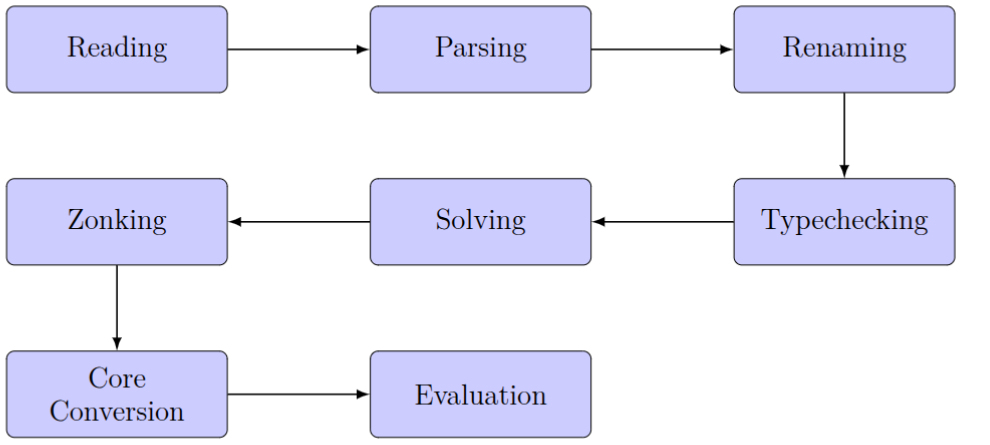
\includegraphics[scale=0.3]{pic/pipeline.png} % You will need a PNG of your pipeline diagram
    \caption{The \texttt{Arralac} Compilation Pipeline. Note the separation of Typechecking (Generation) and Solving.}
  \end{figure}
\end{frame}

\begin{frame}{Core Mechanism: Bidirectional Typechecking}
  The system avoids undecidable inference by operating in two modes.

  \begin{columns}[T]
    \begin{column}{0.5\textwidth}
      \textbf{Inference Mode ($\uparrow$)}
      \begin{itemize}
        \item Synthesizes or "infers" the most general type for an expression.
        \item Used when the type is not known in advance.
        \item For \\ \quad \texttt{let x = \textbackslash x. x} \\ infers \\ \quad \texttt{x :: a -> a}
      \end{itemize}
    \end{column}
    \begin{column}{0.5\textwidth}
      \textbf{Checking Mode ($\downarrow$)}
      \begin{itemize}
        \item Verifies an expression against a known, expected type.
        \item Triggered by programmer annotations.
        \item This is the key to handling higher-rank types.
        \item \texttt{(\textbackslash x. x) :: \\ \quad \quad String -> String}
      \end{itemize}
    \end{column}
  \end{columns}
\end{frame}

\section{Results and Demonstration}

\begin{frame}[containsverbatim]{Positive Case: Higher-Rank Polymorphism}
  The system correctly typechecks a program that passes a polymorphic function as an argument.
  \begin{columns}[T]
    \begin{column}{0.48\textwidth}
      \textbf{Input Code (\texttt{Program1.arralac})}
      \begin{minted}[frame=lines]{haskell}
let
  applyMyShow =
    (\x. \y. x y) ::
      forall a.
        (forall b. b -> String)
        -> a -> String
in
  applyMyShow (\z. "Hello")
        \end{minted}
    \end{column}
    \begin{column}{0.5\textwidth}
      \textbf{Inferred \& Zonked Output (simplified)}
      \begin{minted}[frame=lines,fontsize=\tiny]{haskell}
let
  applyMyShow_0 =
    (\(x_1 :: forall b_4. b_4 -> String).
       (\(y_2 :: a_8).
          (x_1 :: a_8 -> String) 
          (y_2 :: a_8)
       )
    ) :: (forall b_4. b_4 -> String)
       -> a_Unsolved_10 -> String
in
  (applyMyShow_0
     (\(z_8 :: b_11). "Hello")
  ) :: a_Unsolved_10 -> String
        \end{minted}
      \textbf{Result:} Success. The higher-rank annotation guides the typechecker correctly.
    \end{column}
  \end{columns}
\end{frame}

\begin{frame}[containsverbatim]{Negative Case: Skolem Escape Detection}
  The solver correctly rejects invalid programs where a type variable would escape its scope.
  \begin{columns}[T]
    \begin{column}{0.48\textwidth}
      \textbf{Invalid Code (\texttt{Program2.arralac})}
      \begin{minted}[frame=lines]{haskell}
let 
  myRun = 
    \(x :: forall a b. a -> b). 
      (let myBad = \y. y x in myBad)
in
  myRun
        \end{minted}
      This code tries to unify an outer-scope variable with an inner-scope `a`.
    \end{column}
    \begin{column}{0.5\textwidth}
      \textbf{Compiler Error}
      \begin{minted}[fontsize=\scriptsize]{console}
Skolem escape!
The variable:
  a_7[ID 7, L 0, Meta, ...]
has the TcLevel:
  L 0
but the type variable:
  a_11[ID 11, L 1, Meta, ...]
has a larger TcLevel:
  L 1
        \end{minted}
      \textbf{Result:} Correctly rejected. The level-based check works as designed.
    \end{column}
  \end{columns}
\end{frame}

\begin{frame}{Interactive Tooling: The Language Server}
  The LSP brings the type system to life in the editor.
  \begin{figure}
    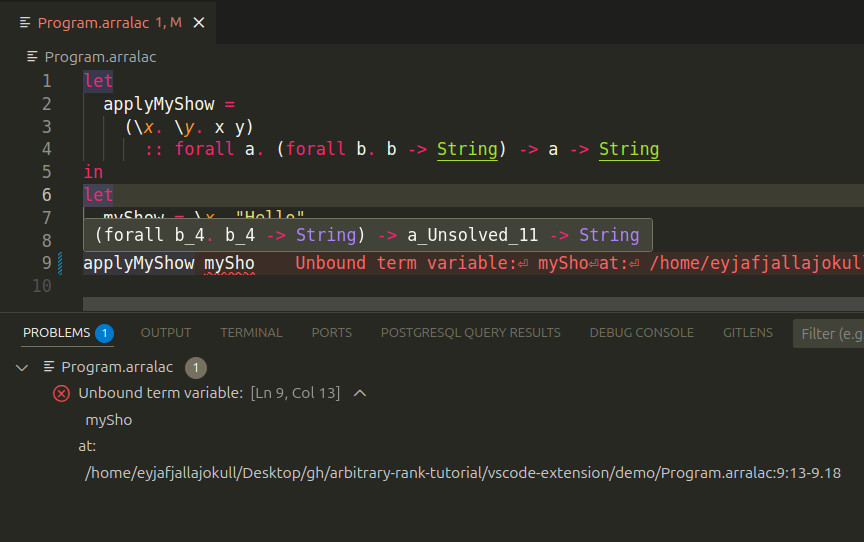
\includegraphics[scale=0.3]{pic/VSCode.png} % Your VS Code screenshot
    \caption{LSP features in VS Code: (1) Type on hover, showing the inferred polymorphic type, and (2) live error diagnostics.}
  \end{figure}
\end{frame}

\section{Conclusion and Future Work}

\begin{frame}{Conclusion}
  \begin{itemize}
    \item \texttt{Arralac} successfully bridges the pedagogical gap between theory and practice for arbitrary-rank polymorphism.
    \item \textbf{Key Insight:} Architectural choices (constraint-based model, TTG, LSP) have a profound impact on a compiler's value as a learning tool.
    \item It demystifies the "magic" by providing a structured, modern, and understandable implementation.
    \item The project provides a clear, interactive bridge for students and aspiring language developers, delivered as a public, open-source repository.
  \end{itemize}
\end{frame}

\begin{frame}{Future Work}
  The tutorial foundation of \texttt{Arralac} enables several clear avenues for future research and development.
  \begin{itemize}
    \item \textbf{Implement \texttt{let}-generalization:} The most significant missing feature. The constraint-based architecture is an ideal foundation for adding scoped constraint solving.

    \item \textbf{Introduce a Typed Core Language:} Evolve the untyped Core language into a typed intermediate representation (like GHC's System FC) to provide end-to-end type safety.

    \item \textbf{Enhance the Constraint Solver:} Improve error reporting to show all residual constraints, not just the first failure. Implement advanced solving strategies like floating constraints.

    \item \textbf{Richer Language Features:} Support user-defined algebraic data types and type classes.
  \end{itemize}
\end{frame}

\begin{frame}
  \begin{center}
    {\Huge Thank You}
    \vspace{2em}

    Questions?

    \vspace{2em}
    Code available at: \url{https://github.com/deemp/arbitrary-rank-tutorial}
  \end{center}
\end{frame}

% \begin{frame}[allowframebreaks]{References}
%   \printbibliography
% \end{frame}

\end{document}